\documentclass[10pt,letterpaper]{article}
\usepackage{spconf,amsmath,amssymb,graphicx,booktabs,url}
\usepackage[T1]{fontenc}
\title{Separating Evidence Freshness, Agent Behavior, and Commit-Time Validity}
\name{Author and affiliation pending}
\address{Development research manuscript --- not submission-ready}
\newcommand{\ind}{\mathbf{1}}
\begin{document}
\maketitle
\begin{abstract}
A successful tool call does not establish that a remembered object binding still satisfies a user's intent. Conversely, a scripted stale-memory failure does not establish that an autonomous language agent will make that mistake. We separate three evidence layers: recorded model behavior, offline execution of a frozen proposed action, and scripted execution-contract tests. In a previously collected ToolSandbox-based diagnostic, three prompting conditions each complete all 14 constructed cases without protocol-defined wrong writes; the inherited-memory baseline already revalidates dynamic targets. We retain this ceiling result rather than claim a benefit from an added verification instruction. Without generating new model responses, we then test state changes at explicit check/use boundaries. All 42 unchanged first-write transitions reproduce; a constructed binding change invalidates 27 dynamic-target actions but none of 15 literal-number actions. A separate 120-trajectory native study illustrates the tradeoff between conservative rejection, predicate scope, and bounded retry. These are conditional mechanism observations, not new live-agent failure rates, a novel concurrency defense, or a demonstration of general safety. The resulting audit identifies which claims are supported and which require independent external evaluation.
\end{abstract}
\begin{keywords}
agent evaluation, memory revalidation, active sensing, execution contracts, reproducibility
\end{keywords}

\section{Introduction and positioning}
A language agent may remember a contact's phone number or an identifier for a reminder. The corresponding database can change while the old value remains syntactically valid. A send operation can therefore succeed at its literal argument while missing a person-oriented goal. Yet constructing such a failure in a fixed script does not show that a language model will blindly reuse the value. An agent may query the current record, making a proposed memory intervention redundant.

The converse distinction is equally important. Fresh evidence can support a decision when read without ensuring that the evidence remains valid when the action executes. A benchmark that changes the environment only before a model episode cannot measure changes between its reads and writes. Rather than infer a broad benefit from one favorable setting, we separate evidence acquisition, autonomous behavior, target binding, and execution-time consistency.

ToolSandbox provides stateful native tools and database snapshots suitable for these diagnostics~\cite{toolsandbox}. Active memory realignment is already studied by GLOVE~\cite{glove}; SafeCommit considers evidence-dependent action certificates and additional probes~\cite{safecommit}. Time-of-check to time-of-use (TOCTOU) risks in language agents and prompt, monitoring, and tool-fusion defenses are explicitly studied by Lilienthal and Hong~\cite{mindgap}. Conditional requests are also an established systems mechanism: HTTP specifies validator-based preconditions such as If-Match~\cite{http}. We do not claim to invent any of these mechanisms.

Our contribution is an auditable diagnostic decomposition with an explicit negative finding: a generic verification instruction does not improve correctness in the tested model setting. We combine that observation with narrowly scoped native execution counterexamples, while preventing offline interventions from being misreported as newly sampled model failures. This manuscript is a development synthesis; its limited task diversity and unestablished algorithmic novelty are not hidden by the conference layout.

\section{Evidence layers and information boundaries}
\subsection{Recorded model diagnostic: R7C1}
The accepted R7C1 protocol (version 1.0.1) uses unchanged ToolSandbox source at commit \texttt{c8571d7} with a restricted native bridge. Its three intent templates are: message a person's current number; message an explicitly supplied literal number; and modify the reminder currently matching an exact description. The first two use contacts and messaging; the third uses reminders. Four variants per template concern stable state, unrelated change, relevant change with old observation, and relevant change with current observation. Two messaging variants additionally disable cellular service. Thus, 14 cases share three templates and two underlying tool domains; they are not 14 unrelated official benchmark tasks.

The three arms are \emph{stateless}, \emph{inherited}, and \emph{resolve-rule}. Stateless removes both historical memory and pre-task observations, so it is an information ablation rather than a length-matched comparison. Inherited receives those materials. Resolve-rule receives the same materials plus a generic instruction to validate dynamic identity or description before writing and to respect literal-number intent. Tool permissions and an eight-request episode cap are shared. All arms use a common instruction noting that historical evidence may be outdated. There is no model user simulator or model judge.

The requested endpoint label is \texttt{deepseek-v4-flash}; recorded responses use \texttt{deepseek-flash}. One smoke establishes the permitted response-label/fingerprint pair, which remains fixed within the batch. This records metadata consistency, not independent verification of the underlying weights. The output cap is 16,384, thinking is enabled, reasoning effort is high, and temperature is omitted. Research cost includes primary, repeated, and smoke calls separately; unknown monetary cost remains unknown.

We preserve the original endpoint: safe success means goal achievement with no wrong write anywhere in the trace. A later correct action does not erase an earlier wrong write. Termination is reported separately rather than inserted into the endpoint after observing results. The 42 primary episodes are the 14 cases under three arms. Six repeated episodes are diagnostics and never replace primary answers.

\subsection{Offline frozen-action exposure: R8A2}
After observing the R7C1 ceiling, we reuse each primary episode's recorded native action prefix up to its first mutating call. We replay that prefix into its original snapshot and keep the already generated mutation arguments fixed. In a control, state is unchanged. In the intervention, the target's current phone mapping or reminder-description binding changes immediately before the write. Literal-number requests retain their explicit number semantics. All 42 primary prefixes are included, yielding 84 transition checks.

There is no post-intervention model continuation: no model is asked to observe, repair, retry, or change its plan. This is a conditional test of a proposed action in a changed prestate, not an on-policy agent evaluation. It cannot estimate how often such changes occur or whether a live agent would subsequently recover. The original 14/14 scores remain unchanged.

\subsection{Scripted execution-contract study: R8A1}
We separately cross three intents with ten event/timing cells: one no-change cell, and unrelated, binding-changing, and non-binding target-field updates placed before resolution, after resolution, or after use. Every cell is tested with four scripted contracts, giving 120 native trajectories. Changes are deliberate simulator interventions, not sampled production incidents. All data remain within simulated contacts, messages, reminders, and settings.

\emph{Query-use} resolves the target and writes without a commit precondition. \emph{Global guard} validates a whole-world snapshot token before the write, rejecting any intervening change. \emph{Scoped guard} checks only the binding required by the declared intent. \emph{Scoped retry} adds at most one re-resolution after a rejected scoped check. All preserve full native traces and report completion, wrong writes, rejections, and reads separately.

For the guarded contracts, check and write form an indivisible segment in a deterministic, cooperating event schedule. This is an additional environment capability, not a prompt improvement or a guarantee that remote APIs support transactions. ToolSandbox's global context is not used as a thread-safe concurrent server. Comparing guards with unguarded calls is therefore a comparison of execution contracts, not equal-capability algorithm superiority.

\section{Correctness conventions and known boundaries}
Let $q$ be a declared intent, $w_c$ the state observed at checking time, and $w_u$ the state immediately before a write. A binding $b(q,w)$ identifies the action target: an identity--number pair for a person, a unique matching reminder identifier for a description, or the supplied literal number. An unchanged literal target need not follow a changed contact record. Let $a$ be the proposed write and $\mathrm{Valid}(q,a,w)$ include the target and permitted state changes.

The relevant implication is not
\begin{equation}
 \mathrm{Valid}(q,a,w_c) \Longrightarrow \mathrm{Valid}(q,a,w_u),
 \label{eq:notimp}
\end{equation}
which need not hold, but an execution contract ensuring validity at the chosen commit point. Repeated non-atomic reads merely move the last observation: when a relevant update remains allowed after that last read, the same construction can invalidate the later write. This is the established TOCTOU boundary, not a new theorem~\cite{mindgap}.

A scoped precondition is sufficient only under explicit assumptions: the intent is correctly specified, the predicate covers all decision-relevant bindings, checking and writing cannot interleave with relevant mutations, and the mutator implements the checked action. If a predicate omits an affected resource or checks a name that is no longer unique, the argument no longer applies. Generic version headers do not automatically establish a multi-resource transaction~\cite{http}.

We score each write relative to its immediate prestate. A change \emph{after} a correctly committed send does not retroactively make it wrong. Conversely, correcting state later does not remove an already committed wrong send. Native reminder creation timestamps may change as documented; unrelated record changes are not permitted agent effects. Environment interventions and agent effects have separate logs.

Rejecting an action can prevent a wrong write without completing the task. Hence our two outputs are
\begin{align}
 S &= \ind\{\text{goal achieved and no wrong write}\},\\
 W &= \ind\{\text{at least one wrong write}\},
\end{align}
with rejection counts and query costs reported alongside them. Zero $W$ alone is not useful-task success. One bounded retry can help for one finished change, but it does not establish liveness under continuing change.

\section{Results}
\subsection{Live-agent ceiling and actual behavior}
Table~\ref{tab:paid} reports primary episodes only. Every arm achieved 14/14 safe success and terminated within the cap. All 15 person-target episodes queried the current contact before sending; all 12 reminder-description episodes queried before modifying. All 15 literal-number episodes honored the requested number. This includes the inherited arm: the stronger instruction did not recover any additional failures.

\begin{table}[t]
\centering\small
\caption{Recorded R7C1 primary results; not R8 model calls.}\label{tab:paid}
\begin{tabular}{lrrrr}
\toprule
Arm & Safe & LLM calls & Tool calls & Input tokens\\
\midrule
Stateless &14/14&51&37&89,224\\
Inherited &14/14&49&35&96,493\\
Resolve-rule &14/14&49&35&100,278\\
\bottomrule
\end{tabular}
\end{table}

The batch contains 149 primary requests, 19 repeated requests, and one smoke: 169 in total. Primary output tokens are 3,669, 4,607, and 3,763 for the three arms. Thus fewer calls did not imply fewer tokens. Money is not inferred from counts. The same initial inputs yielded identical parsed tool-operation sequences in three of six repeated pairs; free-form completion wording differed in all six. All repeated outcomes were safe, but neither text nor generation cost was deterministic.

These results establish a ceiling for this small, explicit protocol, not safety on arbitrary tasks. There is no length-matched placebo for the added instruction, no second endpoint, and no concurrent state change in the original episodes. We do not perform a confirmatory superiority or equivalence test on these cases.

\subsection{Frozen actions expose a different assumption}
All 42 unchanged first-write controls reproduce correct transitions. Under the chosen binding replacement, all 15 person-target and all 12 reminder-target writes become incorrect at that commit point; all 15 literal-number writes remain correct. The total 27 is a count of exposed recorded actions under a constructed intervention. It is \emph{not} 27 newly observed live-model failures, and it must not replace the original all-success score.

This contrast separates current-object intent from literal-argument intent. The tool may execute a literal argument correctly even when a person-based resolution has become stale; the reverse is also possible if a controller overrules the user's explicit number. Freezing the action isolates this interface boundary while deliberately leaving post-change model behavior unmeasured.

\subsection{Execution contracts trade rejection for completion}
\begin{table}[t]
\centering\small
\caption{Scripted contracts over the same 30 cells each. ``Reject'' counts attempts, including retries. Reads/writes are native outer calls; global token operations are additional.}\label{tab:contracts}
\begin{tabular}{lrrrr}
\toprule
Contract & Safe & Wrong & Reject & Calls\\
\midrule
Query-use &28&2&0&50\\
Global guard &21&0&9&41\\
Scoped guard &28&0&2&68\\
Scoped + 1 retry &30&0&2&74\\
\bottomrule
\end{tabular}
\end{table}

Query-use fails in the person and reminder binding-change gaps. It succeeds when changes occur before resolution or after a valid commit, and on literal-number tasks. The global guard avoids wrong writes but rejects nine cells, seven more than the scoped guard. These extra rejections concern conditions that do not invalidate the scoped intent. The scoped guard has two safe non-completions; one retry completes them after the single scheduled change. In two separately retained continuing-change tests, both scoped retries are rejected and no write is performed. They are not added to Table~\ref{tab:contracts}.

The global guard additionally issues and checks 30 whole-state tokens. Preparation uses two native queries per freshly constructed trajectory and is reported separately. Outer-call totals do not measure internal nested calls, remote requests, fees, or a universal cost advantage. In particular, the guarded contracts obtain correctness from their stipulated check/write semantics; no learned optimizer has outperformed a same-capability baseline.

\begin{figure}[t]
\centering
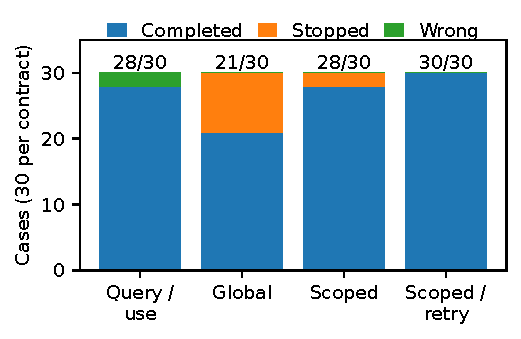
\includegraphics[width=\columnwidth]{figures/contract_outcomes.pdf}
\caption{Completion and failure must be separated. Scripted interleaving coverage is not an estimate of deployed event frequencies.}\label{fig:contracts}
\end{figure}

\section{Reproducibility, limitations, and decision}
The prior batch retains raw requests, responses, state transitions, source hashes, and separate primary/repeat ledgers. We independently recomputed its 48 episode scores and 169 request accounting records without model calls. For the new native study, 36 unit/integration tests include wrong-target, unintended-effect, post-commit-change, retry-exhaustion, and network-blocking cases. Repeating all 120 contracts yields the same discrete scientific projection; native identifiers, creation times, and elapsed times remain in raw traces rather than being claimed byte-identical. All new execution is offline. These checks are from one research assistant, not an independent human replication.

The work has three material limits. First, the original prompt explicitly warns about outdated evidence and identifies current-target intent, so its ceiling is not representative of underspecified language tasks. Second, the new interleavings are constructed after inspecting that ceiling; there is no prospective preregistration, frequency estimate, or measured live-agent adaptation. Third, atomic guards are environment assumptions. A fused function is not necessarily atomic across remote services, and a resource version can miss dependencies outside its scope. We preserve the original ToolSandbox implementation and label our added contracts separately.

Earlier development on calibration and scheduling remains separate: its objectives, tasks, and unit costs changed across rounds. Its negative outcomes do not become evidence for a new guard, and neither this diagnostic nor a formatting revision validates the separate RepairLens project. The present manuscript therefore does not claim a state-of-the-art method or submission readiness.

\section{Conclusion}
The available evidence favors disciplined separation rather than a universal memory-maintenance claim. A live agent can avoid a scripted stale-binding failure by querying, while a correctly queried binding can still become invalid before use. Basic scoped checks can avoid irrelevant global rejections, but their protection depends on executable consistency contracts and bounded-change assumptions. Further paid-model experiments are justified only by a new external task or capability question that these controls cannot already answer; merely expanding the current ceiling cases is not such a question.

\section{Acknowledgment}
ChatGPT was used for research code, test design, analysis, figures, and English drafting. The previously recorded endpoint supplied the R7C1 responses; no new LLM responses were generated for the R8 experiments. Human author attribution, independent review, and final submission checks remain pending.

\begin{thebibliography}{9}
\bibitem{toolsandbox} J. Lu et al., ``ToolSandbox: A Stateful, Conversational, Interactive Evaluation Benchmark for LLM Tool Use Capabilities,'' arXiv:2408.04682, 2024.
\bibitem{glove} X. Yin and H. Du, ``GLOVE: Global Verifier for LLM Memory-Environment Realignment,'' arXiv:2601.19249, 2026.
\bibitem{safecommit} M. Akewar and R. Ranjan, ``SafeCommit: Certifying When Memory-Grounded Agents May Safely Act,'' arXiv:2608.04289, 2026.
\bibitem{mindgap} D. Lilienthal and S. Hong, ``Mind the Gap: Time-of-Check to Time-of-Use Vulnerabilities in LLM-Enabled Agents,'' arXiv:2508.17155, 2025.
\bibitem{http} R. Fielding, M. Nottingham, and J. Reschke, ``HTTP Semantics,'' RFC 9110, June 2022, Secs. 13.1.1 and 13.2.
\end{thebibliography}
\end{document}
